\section{Exercise 15 from TAOCP ``7.1.3 Bitwise tricks and techniques''}

\renewcommand{\CURPATH}{equations/TAOCP_7_1_3_exercise_15}

Page 53 from the fasc1a.ps, or: \url{http://www.cs.utsa.edu/~wagner/knuth/fasc1a.pdf}

\begin{figure}[H]
\centering
\frame{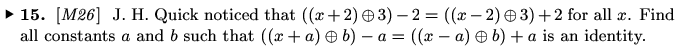
\includegraphics[scale=0.6]{\CURPATH/page53.png}}
\caption{Page 53}
\end{figure}

Soltuion:

\lstinputlisting[style=custompy]{\CURPATH/exercise_15.py}

For 4-bit bitvectors:

\begin{lstlisting}

...

[b = 7, a = 0]
[b = 6, a = 8]
[b = 7, a = 8]
[b = 6, a = 12]
[b = 7, a = 12]
[b = 12, a = 0]
[b = 13, a = 0]
[b = 12, a = 8]
[b = 13, a = 8]
[b = 12, a = 4]
[b = 13, a = 4]
[b = 12, a = 12]
[b = 13, a = 12]
[b = 14, a = 0]
[b = 15, a = 0]
[b = 14, a = 4]
[b = 15, a = 4]
[b = 14, a = 8]
[b = 15, a = 8]
[b = 14, a = 12]
[b = 15, a = 12]
results total= 128
\end{lstlisting}

